% !TEX program = pdflatex
% ================================================================
% COMET -- ICLR 2027 working draft
% ================================================================
% Submission mode is anonymous by default. For camera-ready only:
%   \iclrfinalcopy
% The exact official 2027 style files should replace the local copies
% before submission. See STYLE_NOTICE.md.
% ================================================================

\documentclass{article}

\usepackage{iclr2027_conference,times}
\usepackage{amsmath,amssymb,amsthm,mathtools,bm}
\usepackage{booktabs,multirow,array,tabularx}
\usepackage{algorithm}
\usepackage{algpseudocode}
% Make hyperref destinations for algorithmic lines unique across algorithms.
\makeatletter
\renewcommand{\theHALG@line}{\thealgorithm.\arabic{ALG@line}}
\makeatother
\usepackage{graphicx}
\usepackage{microtype}
\usepackage{xcolor}
\usepackage{enumitem}
\usepackage{tikz}
\usetikzlibrary{arrows.meta,positioning,fit,calc}
\usepackage{url}
\usepackage{hyperref}
\usepackage[nameinlink,capitalise,noabbrev]{cleveref}
\hypersetup{colorlinks=true,linkcolor=blue!55!black,citecolor=blue!55!black,urlcolor=blue!55!black}

% Core notation. Keep this file small to avoid accidental conflicts.
\newcommand{\E}{\mathbb{E}}
\newcommand{\Prb}{\mathbb{P}}
\newcommand{\Var}{\operatorname{Var}}
\newcommand{\Cov}{\operatorname{Cov}}
\newcommand{\ind}{\mathbf{1}}
\newcommand{\R}{\mathbb{R}}
\newcommand{\F}{\mathcal{F}}
\newcommand{\Hcal}{\mathcal{H}}
\newcommand{\Qcal}{\mathcal{Q}}
\newcommand{\Scal}{\mathcal{S}}
\newcommand{\Ical}{\mathcal{I}}
\newcommand{\Bcal}{\mathcal{B}}
\newcommand{\Gcal}{\mathcal{G}}
\newcommand{\Pcal}{\mathcal{P}}
\newcommand{\Mcal}{\mathcal{M}}
\newcommand{\abs}[1]{\left|#1\right|}
\newcommand{\norm}[1]{\left\lVert#1\right\rVert}
\newcommand{\ip}[2]{\left\langle#1,#2\right\rangle}
\newcommand{\given}{\,\middle|\,}
\newcommand{\op}{\mathrm{op}}
\newcommand{\eff}{\mathrm{eff}}
\newcommand{\dep}{\mathrm{dep}}
\newcommand{\nuis}{\mathrm{nuis}}
\newcommand{\coup}{\mathrm{coup}}
\newcommand{\drift}{\mathrm{drift}}
\newcommand{\MOM}{\operatorname{MOM}}
\newcommand{\LCB}{\operatorname{LCB}}
\newcommand{\UCB}{\operatorname{UCB}}
\newcommand{\polylog}{\operatorname{polylog}}
\newcommand{\COMET}{\textsc{Comet}}
\DeclareMathOperator*{\argmax}{arg\,max}
\DeclareMathOperator*{\argmin}{arg\,min}


% Draft annotations are intentionally disabled in the compiled paper.
% Change to \showdraftnotestrue while developing.
\newif\ifshowdraftnotes
\showdraftnotesfalse
\newcommand{\draftnote}[1]{\ifshowdraftnotes\par\noindent\fcolorbox{orange!70!black}{orange!8}{\parbox{0.95\linewidth}{\textbf{Draft note.} #1}}\par\fi}
\newcommand{\todo}[1]{\ifshowdraftnotes\textcolor{red!70!black}{[TODO: #1]}\fi}

\theoremstyle{plain}
\newtheorem{theorem}{Theorem}[section]
\newtheorem{proposition}[theorem]{Proposition}
\newtheorem{lemma}[theorem]{Lemma}
\newtheorem{corollary}[theorem]{Corollary}
\theoremstyle{definition}
\newtheorem{definition}[theorem]{Definition}
\newtheorem{assumption}[theorem]{Assumption}
\theoremstyle{remark}
\newtheorem{remark}[theorem]{Remark}
\newtheorem{example}[theorem]{Example}

\title{\COMET: Counterfactual Moment Auditing\\under Weak Overlap and Dependent Feedback}

\author{Anonymous Authors}

\begin{document}
\maketitle

\begin{abstract}
Logged decision systems increasingly combine learned policies, adaptive data collection, and interacting units. Their counterfactual statistics can be unstable for three distinct reasons: target and logging policies may have only weak overlap, outcomes may be heavy-tailed, and observations may be dependent through repeated users, slates, networks, or temporal feedback. We introduce \COMET, a general framework for estimating and testing families of counterfactual moments in this regime. The framework begins with an orthogonal score that covers off-policy value, subgroup effects, counterfactual calibration, safety constraints, and exposure-mediated spillovers. It then combines dependence-separated cross-fitting with graph--time robust aggregation to produce simultaneous certificates over target policies and auditors. The proposed rate separates heavy-tail difficulty, an observable conflict-graph design effect, nuisance-estimation error, temporal coupling, and within-window drift. Building on these certificates, we formulate a discover--certify procedure for finding hidden failure subgroups without reusing the certification data, and a pessimistic policy-repair rule with high-probability feasibility. We specify a complete empirical program spanning controlled synthetic processes, semi-synthetic temporal graphs, and real logged recommendation data. The resulting problem is broader than counterfactual fairness on evolving graphs: that setting is recovered as one instance of a common counterfactual-moment interface.
\end{abstract}

\paragraph{Gate A scope notice.}
The abstract and original sections describe the broader research program.
The proved certificate in this audited draft is \cref{thm:gate-a-clean}:
a fixed-design, independent-evaluation-block result with explicit constants
and known moment envelopes. The original adaptive-history and mutually
cross-fitted concentration claims remain unproved outside that model.
The corrected lower bound concerns exact clique replication and expected
absolute risk. No final empirical coverage or long-run deployment-safety
claim is established by this first-stage audit.


\section{Introduction}
\label{sec:intro}

Logged decision systems increasingly learn from data generated by earlier versions of themselves. A logging policy selects an exposure, only the corresponding outcome is observed, and the resulting log is reused to evaluate or constrain a target policy. The relevant questions extend beyond average policy value: is a score calibrated under an intervention, does a policy violate a safety constraint, are direct or spillover effects unequal across subgroups, and can a hidden failure population be detected? Each can be expressed as a \emph{counterfactual moment}: an intervention-specific orthogonal score multiplied by an auditor or constraint function.

Reliable inference is difficult when three pathologies interact. \emph{Weak overlap} produces large importance ratios for actions rarely chosen by the logging policy, even with bounded rewards. Outcomes such as watch time, transaction value, and medical cost may themselves be heavy-tailed. Finally, units are dependent through shared slates, repeated users, local interference, and temporal feedback. Doubly robust estimation \citep{dudik2011doubly,jiang2016doubly,farajtabar2018more}, weak-overlap analysis \citep{wang2017optimal,mehrabi2024weak,khan2024beyond}, robust mean estimation \citep{lugosi2019mean}, and causal inference under interference \citep{aronow2017estimating,savje2021average} address important parts of this problem, but do not by themselves provide simultaneous, operational certificates for families of counterfactual questions in dependent logs.

We introduce \textbf{\COMET} (\textbf{CO}unterfactual \textbf{M}oment \textbf{E}stimation and \textbf{T}esting). A generalized exposure mapping converts a joint assignment into a local exposure state; a cross-fitted orthogonal score identifies a target intervention; a logged conflict graph records dependence induced by slates, entities, and declared interference neighborhoods; and graph--time median-of-means aggregation produces simultaneous confidence radii under only a finite $p$th moment, $p\in(1,2]$. The target is a predictable window average, so adaptive deployment and within-window drift are visible rather than hidden inside a stationary population mean.

\begin{figure}[t]
  \centering
  \resizebox{\linewidth}{!}{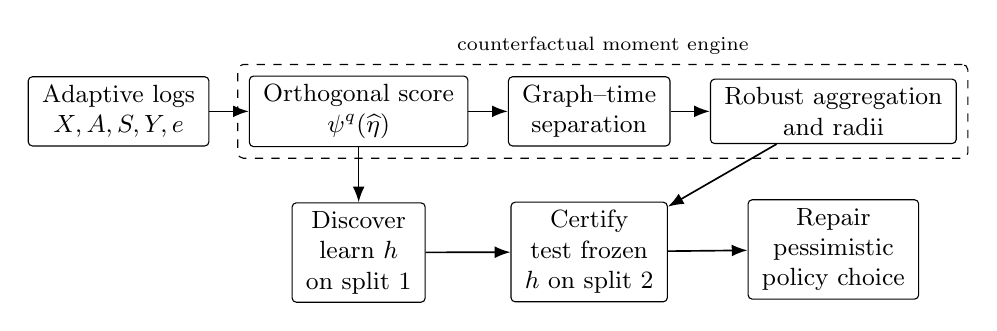
\begin{tikzpicture}[
  node distance=5mm and 5mm,
  box/.style={draw,rounded corners=1.5pt,align=center,minimum height=8mm,inner xsep=5pt,inner ysep=3pt,font=\small},
  arrow/.style={-{Latex[length=2mm]},semithick},
  group/.style={draw,dashed,rounded corners=2pt,inner sep=4pt}
]
\node[box] (log) {Adaptive logs\\$X,A,S,Y,e$};
\node[box,right=of log] (score) {Orthogonal score\\$\psi^q(\widehat\eta)$};
\node[box,right=of score] (split) {Graph--time\\separation};
\node[box,right=of split] (robust) {Robust aggregation\\and radii};
\draw[arrow] (log) -- (score);
\draw[arrow] (score) -- (split);
\draw[arrow] (split) -- (robust);

\node[box,below=7mm of score] (discover) {Discover\\learn $h$ \\ on split 1};
\node[box,below=7mm of split] (certify) {Certify\\test frozen \\ $h$ on split 2};
\node[box,below=7mm of robust] (repair) {Repair\\pessimistic\\ policy choice};
\draw[arrow] (score) -- (discover);
\draw[arrow] (discover) -- (certify);
\draw[arrow] (robust) -- (certify);
\draw[arrow] (certify) -- (repair);

\node[group,fit=(score)(split)(robust),label={[font=\scriptsize]above:counterfactual moment engine}] {};
\end{tikzpicture}
}
  \caption{\COMET separates counterfactual scoring, dependence-aware robust inference, and downstream use. Auditors may be learned on a discovery split, but certification and policy repair use a separate graph--time split.}
  \label{fig:overview}
\end{figure}

The certificates support a \emph{discover--certify--repair} workflow (\cref{fig:overview}). A flexible auditor searches for a violating subgroup on one split and is frozen before testing on a dependence-separated certification split. Certified upper and lower bounds are then used for pessimistic policy selection: optimize a utility lower confidence bound while enforcing risk, fairness, or resource upper confidence bounds.

\paragraph{Contributions.}
\begin{enumerate}[leftmargin=1.35em,itemsep=1pt,topsep=2pt]
    \item We give one counterfactual-moment interface covering off-policy and subgroup value, intervention-specific calibration, heterogeneous effects, safety constraints, and local spillovers.
    \item We propose graph--time separated cross-fitting and robust aggregation. The main bound separates a heavy-tail term of order $N_{\eff}^{-(p-1)/p}$, an observable conflict-graph design effect, nuisance bias, temporal coupling, and drift. A cluster construction gives a matching dependence--tail lower bound up to logarithms.
    \item We develop learn-then-certify subgroup auditing, ratio certificates that account for denominator uncertainty and abstain under insufficient support, and pessimistic policy repair with high-probability feasibility.
    \item We specify coverage-centered experiments on controlled dynamic processes, real temporal-graph structures, Open Bandit, and KuaiRand, with separate stress tests for weak overlap and heavy-tailed outcomes.
\end{enumerate}

Counterfactual online performative fairness (COPF) on evolving graphs \citep{li2026copf} is recovered by choosing shown/not-shown exposure, group--score auditors, and exposure-effect constraints. Here it is one instance rather than the paper's organizing premise: strict overlap is replaced by finite-moment weak overlap, fixed slices are augmented by learned auditors, and generic online control is replaced by certificate-guided repair.

\section{Counterfactual Moments from Adaptive Dependent Logs}
\label{sec:setup}

At round $t$, the system observes history $\F_{t-1}$ and units $\Ical_t$, then draws a possibly joint action $A_t$. For $u=(t,i)$ with context $X_u$, a known exposure mapping
\begin{equation}
S_u=g_u(A_{I(u)})\in\Scal
\label{eq:exposure-map}
\end{equation}
compresses the relevant assignment into a finite local state (e.g., shown/not shown, slate position, or treatment plus neighbor exposure). Let $Y_u(s)$ be the potential outcome and $Y_u=Y_u(S_u)$. Define
\begin{equation}
e_u(s)=\Prb(S_u=s\mid X_u,\F_{t-1}),\qquad
\mu_u(s)=\E[Y_u(s)\mid X_u,\F_{t-1}].
\label{eq:nuisance}
\end{equation}
A predictable target intervention $q\in\Qcal$ assigns mass $q_u(s\mid X_u,\F_{t-1})$.

\begin{assumption}[Local identification]
\label{ass:identification}
Consistency holds through \cref{eq:exposure-map}; $Y_u(s)\perp S_u\mid X_u,\F_{t-1}$; and $q_u(s)>0$ implies $e_u(s)>0$ almost surely.
\end{assumption}
This is support positivity, not a uniform lower bound. The generalized doubly robust score is
\begin{equation}
\psi_u^q(\eta)=\sum_{s\in\Scal}q_u(s)
\left[\mu_u(s)+\frac{\ind\{S_u=s\}}{e_u(s)}\{Y_u-\mu_u(s)\}\right],
\label{eq:orthogonal-score}
\end{equation}
where $\eta=(\mu,e)$. For auditor $h\in\Hcal$, predictable reference $f_u$, and window $\Ical_W$ of size $N_W$, we target the pathwise predictable moment
\begin{equation}
M_W(q,h;f)=\frac1{N_W}\sum_{u\in\Ical_W}
\E[h_u\{\psi_u^q(\eta_0)-f_u\}\mid\F_{t(u)-1}].
\label{eq:target-moment}
\end{equation}
Unlike a stationary estimand, \cref{eq:target-moment} follows the realized deployment path.

\begin{proposition}[Identification and double robustness]
\label{prop:dr}
Under \cref{ass:identification}, $\E[\psi_u^q(\eta_0)\mid X_u,\F_{t-1}]=\sum_s q_u(s)\mu_u(s)$. For generic $\bar\eta=(\bar\mu,\bar e)$,
\begin{equation}
\E[\psi_u^q(\bar\eta)-\psi_u^q(\eta_0)\mid X_u,\F_{t-1}]
=\sum_s q_u(s)\{\bar\mu_u(s)-\mu_u(s)\}
\frac{\bar e_u(s)-e_u(s)}{\bar e_u(s)}.
\label{eq:dr-remainder}
\end{equation}
\end{proposition}

\begin{table}[t]
\centering\small
\setlength{\tabcolsep}{3.5pt}
\begin{tabularx}{\linewidth}{@{}p{.25\linewidth}p{.28\linewidth}X@{}}
\toprule
Question & $(q,f)$ & Auditor / contrast \\
\midrule
Policy or subgroup value & target policy, $f=0$ & $h=1$ or subgroup indicator \\
Counterfactual calibration & intervention, $f=\widehat p$ & group/score tests or learned $h$ \\
Heterogeneous effects & $\psi^{q_1}-\psi^{q_0}$ & group, role, or learned subgroup \\
Safety / spillovers / COPF & cost or local exposure state & one-sided constraints or parity tests \\
\bottomrule
\end{tabularx}
\caption{Representative instantiations; details are in \cref{app:examples}.}
\label{tab:moment-examples}
\end{table}

\paragraph{Weak overlap and heavy tails.}
For some $p\in(1,2]$, assume uniformly over $(q,h)$
\begin{equation}
\frac1{N_W}\sum_u\E[|h_u\{\psi_u^q(\eta_0)-f_u\}|^p\mid\F_{t(u)-1}]\le\nu_p^p.
\label{eq:p-moment}
\end{equation}
\begin{assumption}[Finite-$p$ score moments]
\label{ass:p-moment}
Equation~\eqref{eq:p-moment} holds for the oracle score; the theorem additionally requires the centered cross-fitted score to obey a stated conditional envelope.
\end{assumption}
A sufficient residual condition contains $q_u(s)^p e_u(s)^{1-p}\E[|Y_u(s)-\mu_u(s)|^p\mid X_u,\F_{t-1}]$, exposing separate failure modes from small propensities and heavy-tailed outcomes.

\paragraph{Observable dependence and drift.}
Construct a conflict graph $G_W$ on audited units: connect units sharing randomized exposure, a slate, repeated entity, outcome shock, or declared interference neighborhood. In temporal block $b$, let $\chi_b$ be a proper-coloring count. Blocks are separated by a gap $\ell$; an offline coupling fails with probability at most $\varepsilon_{\coup}$, while adaptive analysis conditions on the past. Nonstationarity is measured by
\begin{equation}
\Delta_W(q,h)=\max_{b\le B}|M_b(q,h)-M_W(q,h)|.
\label{eq:drift}
\end{equation}
Thus window length trades effective sample size against drift.

\section{The \COMET\ Estimator}
\label{sec:method}

\COMET separates nuisance learning, dependence control, and heavy-tail robustification. This permits independent diagnostics of propensity support, outcome-model error, conflict-graph inflation, and tail sensitivity.

\paragraph{Dependence-separated cross-fitting.}
Random row-wise folds leak information when rows share a user, slate, neighborhood, or nearby latent state. We form evaluation folds from time macro-blocks with guard gaps and prohibited-entity separation. For unit $u$ in fold $k(u)$, nuisances are trained only on allowed blocks and the score is
\begin{equation}
\widehat Z_u(q,h)=h_u\{\psi_u^q(\widehat\eta^{(-k(u))})-f_u\}.
\label{eq:crossfit-score}
\end{equation}
Fold construction uses design variables available before observing outcomes. When exact logging propensities are available, only $\mu$ is learned and the propensity component of the double-robust remainder is zero.

\paragraph{Graph--time median of means.}
Retain $B$ temporally separated blocks of common size $n_0$, so $N_W=Bn_0$. Properly color each block conflict graph, set $\bar\chi_W=\max_b\chi_b$, and define the conservative effective sample size
\begin{equation}
N_{\eff}=N_W/\bar\chi_W.
\label{eq:neff}
\end{equation}
For each $\theta=(q,h)$, compute block means $\bar Z_b(\theta)=n_0^{-1}\sum_{u\in b}\widehat Z_u(\theta)$. Partition the $B$ blocks into $K$ equal-count super-blocks, average within each super-block, and take
\begin{equation}
\widehat M_W(\theta)=\operatorname{median}_{g\le K}
\left\{\frac1{|g|}\sum_{b\in g}\bar Z_b(\theta)\right\}.
\label{eq:comet-estimator}
\end{equation}
Equal block sizes preserve the raw-unit target; variable-size extensions and a streaming truncation variant appear in the appendix.

\begin{algorithm}[t]
\caption{\COMET\ certification for finite $\Theta=\Qcal\times\Hcal$}
\label{alg:comet}
\begin{algorithmic}[1]
\Require Logs, exposure map, policies $\Qcal$, auditors $\Hcal$, confidence $\delta$.
\State Build guarded time blocks and logged conflict graphs; create separated cross-fitting folds.
\State Fit $\widehat\eta^{(-k)}$ and compute $\widehat Z_u(q,h)$ for all $(q,h)\in\Theta$.
\State Color each block, compute $N_{\eff}$, and aggregate by \cref{eq:comet-estimator}.
\State Form simultaneous radii with tail, nuisance, coupling, and drift terms.
\State \Return intervals, $N_{\eff}$, overlap/tail diagnostics, and support-based abstentions.
\end{algorithmic}
\end{algorithm}

\paragraph{Radius decomposition.}
The working radius is
\begin{equation}
\begin{split}
r_W(q,h;\delta)={}&C_p\widehat\nu_p(q,h)
\left(\frac{\log(2|\Theta|/\delta)}{N_{\eff}}\right)^{\frac{p-1}{p}}
+r_{\nuis}(q,h)\\
&+r_{\coup}(q,h)+r_{\drift}(q,h).
\end{split}
\label{eq:radius}
\end{equation}
The terms answer different operational questions: insufficient support/tail mass, nuisance misspecification, inadequate time separation, or an overly long window. For estimated propensities, the exact bias is bounded by
\begin{equation}
R_{\nuis}(q,h)=\frac1{N_W}\sum_u\E\!\left[
|h_u|\sum_s q_u(s)|\widehat\mu_u(s)-\mu_u(s)|
\frac{|\widehat e_u(s)-e_u(s)|}{\widehat e_u(s)}\right].
\label{eq:nuisance-rem}
\end{equation}
A valid certificate must use either exact propensities/one correct nuisance or a justified high-probability upper bound $r_{\nuis}\ge R_{\nuis}$; a plug-in diagnostic alone is not a proof of coverage.

\paragraph{Ratio certificates and abstention.}
For a subgroup ratio $|m_h|/\pi_h$, construct simultaneous radii $r_{m,h}$ and $r_{\pi,h}$. If $\widehat\pi_h-r_{\pi,h}>0$, then
\begin{equation}
\frac{|m_h|}{\pi_h}\le
\frac{|\widehat m_h|+r_{m,h}}{\widehat\pi_h-r_{\pi,h}}.
\label{eq:ratio-cert}
\end{equation}
Otherwise \COMET\ returns \emph{insufficient support to certify}. This prevents tiny slices from receiving precise-looking but unsupported calibration or fairness scores.

\paragraph{Tail tuning.}
The clean theorem treats $p$ and an envelope $\nu_p$ as known. Experiments compare oracle tuning, a sensitivity grid whose intervals are unioned, and an adaptive Lepski-style rule. Only variants with a proved or separately validated tuning guarantee are presented as confidence procedures.

\section{Finite-Sample Guarantees}
\label{sec:theory}

We state the core result for a finite family $\Theta=\Qcal\times\Hcal$; the certification stage of a learned auditor is finite because the discovered tests are frozen before evaluation.

\begin{lemma}[Conflict-graph moment reduction]
\label{lem:graph-moment}
Let $X_1,\ldots,X_n$ be conditionally mean-zero with a conditional dependency graph admitting a proper coloring with $\chi$ colors. If $p\in(1,2]$ and $\E[|X_i|^p\mid\mathcal D]\le\nu^p$, then
\begin{equation}
\E\!\left[\left|\frac1n\sum_{i=1}^nX_i\right|^p\middle|\mathcal D\right]
\le C_p\nu^p\left(\frac{\chi}{n}\right)^{p-1}.
\label{eq:graph-moment}
\end{equation}
\end{lemma}
The proof colors the graph, applies the von Bahr--Esseen inequality within independent color classes, and combines color sums by convexity (\cref{app:proof-graph}). Thus $n/\chi$ acts as a conservative effective sample size.

Let retained blocks have size $n_0$, coloring count at most $\bar\chi_W$, and total coupling failure $\varepsilon_{\coup}$. Split $B$ blocks into $K$ MOM super-blocks.

\begin{theorem}[Uniform \COMET\ certificate]
\label{thm:uniform-comet}
Suppose \cref{ass:identification,ass:p-moment} hold; cross-fitting is dependence-separated; the centered cross-fitted scores satisfy the conditional $p$-moment envelope $\nu_p$; and \cref{lem:graph-moment} applies within each block. Let
\begin{equation*}
K=\left\lceil8\log\frac{2|\Theta|}{\delta}\right\rceil\le B/2.
\end{equation*}
If $r_{\nuis}\ge R_{\nuis}^{\star}$ is a valid simultaneous nuisance-bias bound, then with probability at least $1-\delta-\varepsilon_{\coup}$,
\begin{equation}
\sup_{\theta\in\Theta}|\widehat M_W(\theta)-M_W(\theta)|
\le C_p\nu_p\left(
\frac{\log(2|\Theta|/\delta)}{N_{\eff}}
\right)^{\frac{p-1}{p}}
+r_{\nuis}+\Delta_W^{\star},
\label{eq:main-bound}
\end{equation}
where $\Delta_W^{\star}=\sup_{\theta}\Delta_W(\theta)$. With exact block independence and stable targets, the coupling failure and drift correction vanish.
\end{theorem}

At $p=2$, the stochastic term is $N_{\eff}^{-1/2}$ up to logarithms; for $p<2$, it is $N_{\eff}^{-(p-1)/p}$. The proof conditions on design and nuisance-training data, applies \cref{lem:graph-moment} to each block, averages independent coupled blocks inside super-blocks, and uses a majority argument plus a union bound over $\Theta$. Equation~\eqref{eq:dr-remainder} supplies the nuisance product term, and nonidentical block targets cost at most $\Delta_W^{\star}$. Full details are in \cref{app:proof-main}.

\begin{corollary}[Certified ratios]
\label{cor:ratio}
On the event in \cref{thm:uniform-comet}, every ratio $|m_h|/\pi_h$ obeys \cref{eq:ratio-cert} when the subgroup-mass lower confidence bound is positive; otherwise the data justify only abstention.
\end{corollary}

\paragraph{Lower bound.}
The dependence penalty is not only a proof artifact. Consider $N/\chi$ independent clusters, each replicated exactly $\chi$ times.
\begin{theorem}[Cluster-replication lower bound]
\label{thm:lower}
For $p\in(1,2]$ and $\chi\mid N$, over distributions satisfying $\E|X-\E X|^p\le\nu_p^p$ under the cluster model, every estimator $\widetilde M$ obeys
\begin{equation}
\inf_{\widetilde M}\sup_P\E_P|\widetilde M-M(P)|
\ge c_p\nu_p\left(\frac{\chi}{N}\right)^{\frac{p-1}{p}}.
\label{eq:lower-bound}
\end{equation}
\end{theorem}
The proof reduces to finite-$p$ mean estimation from $N/\chi$ independent samples using a two-point construction (\cref{app:lower}). Hence the tail--dependence interaction in \cref{eq:main-bound} is minimax unavoidable for this general class, up to logarithmic factors. Sharper fractional-coloring parameters remain possible under additional graph structure.

\paragraph{Scope.}
The theorem certifies an identified moment; it cannot test ignorability or an incorrect exposure mapping from logs alone. Estimated propensities require a defensible nuisance bound, and adaptive tail tuning requires its own validity argument. These are explicit assumptions rather than hidden implementation choices.

\section{Discover, Certify, and Repair}
\label{sec:discover-repair}

\paragraph{Learn then certify.}
Fixed score bins can miss failures defined by interactions among group, activity, device, time, and graph position. On a discovery split, fit a rich auditor by
\begin{equation}
\widehat h\in\argmax_{h\in\Hcal_{\rm rich}}
|\widehat M_{\rm disc}(q,h)|-\lambda\Omega(h),
\label{eq:auditor-learning}
\end{equation}
subject to a minimum-support rule. The auditor's parameters and human-readable definition are then frozen. Nuisances and scores are recomputed using only training data allowed for a graph--time separated certification split, where \COMET\ tests $\widehat h$. Conditional on discovery data, the selected auditor is fixed; certifying the top $L$ frozen candidates pays only $\log L$ in the finite-family radius. This separates \emph{finding a suspicious pattern} from \emph{showing that fresh dependent data support it counterfactually}.

\paragraph{Pessimistic policy repair.}
Let $V(q)$ be utility and $C_j(q)$, $j\le J$, be risk, cost, calibration, spillover, or fairness moments with limits $\alpha_j$. Suppose simultaneous estimates satisfy
\begin{equation}
|\widehat V(q)-V(q)|\le r_V(q),\qquad
|\widehat C_j(q)-C_j(q)|\le r_j(q)
\label{eq:sim-policy-event}
\end{equation}
for all policies in a frozen library $\Qcal$. Choose
\begin{equation}
\widehat q\in\argmax_{q\in\Qcal}\{\widehat V(q)-r_V(q)\}
\quad\text{s.t.}\quad
\widehat C_j(q)+r_j(q)\le\alpha_j\quad\forall j.
\label{eq:policy-repair}
\end{equation}
The library may include the deployed policy, exploration mixtures, threshold/group-offset variants, and candidates produced by an unconstrained learner; only the frozen library is covered by the simultaneous theorem.

\begin{proposition}[Feasibility and utility]
\label{prop:repair}
On the event \eqref{eq:sim-policy-event}, every solution of \cref{eq:policy-repair} satisfies $C_j(\widehat q)\le\alpha_j$. For any comparator $q$ with $C_j(q)+2r_j(q)\le\alpha_j$ for all $j$,
\begin{equation}
V(\widehat q)\ge V(q)-2r_V(q).
\label{eq:repair-utility}
\end{equation}
\end{proposition}
The robust margin is substantive: a policy estimated exactly at a constraint boundary cannot be certified without more information. As support improves and $N_{\eff}$ grows, the certified feasible set expands. Sequential deployment repeats the procedure by epoch with an explicit error-spending schedule and never reuses a discovery split as certification data.

\section{Experimental Design}
\label{sec:experiments}

The empirical claim is reliable certification, not minimum point error in one simulator. We ask whether intervals attain nominal coverage; errors scale with $N_{\eff}^{-(p-1)/p}$; graph, time, robustification, and nuisance separation matter in the regimes they target; hidden subgroups can be discovered and replicated; and pessimistic repair improves the utility--constraint frontier.

\paragraph{Controlled dynamic process.}
We use a dynamic degree-corrected block model and a preferential-attachment stream. A logging policy selects an item or Top-$K$ slate via
\begin{equation}
\pi_t=(1-\epsilon_{\rm exp})\operatorname{Softmax}(s_t/\tau)
+\epsilon_{\rm exp}\operatorname{UniformTopK},
\label{eq:synthetic-policy}
\end{equation}
and a sticky latent regime induces temporal persistence. Outcomes follow
\begin{equation}
Y_u=\mu(X_u,Z_t)+\tau_{G_u}A_u+\rho_{G_u}\bar A_{N(u),t}
+b_{\mathrm{entity}(u)}+\varepsilon_u,
\label{eq:synthetic-outcome}
\end{equation}
with direct and spillover effects, repeated-entity dependence, and Gaussian, Student-$t$, or Pareto/Lomax noise. Four regimes separate light tails, weak overlap only, outcome tails only, and both. Sweeps vary sample size, $p$, exploration, candidate budget, hub strength, interference radius, temporal persistence, auditor count, and nuisance misspecification. Ground truth is analytic or obtained from an independent intervention run whose Monte Carlo error is negligible relative to interval width. The key log--log plot compares scaling against raw $N$ and against $N_{\eff}$.

\paragraph{Complementary real-data studies.}
TGB preserves real temporal-graph structure while the logging policy and potential outcomes are simulated, yielding exact counterfactual truth with realistic conflict graphs \citep{huang2023tgb}. Open Bandit uses real propensities and multiple behavior policies; one policy's log evaluates another whose on-policy mean supplies an external target, isolating importance-ratio tails with mostly binary rewards \citep{saito2021open}. KuaiRand adds repeated-user sequences, randomized exposures, and heavy-tailed watch time; its randomized portion supports held-out intervention checks, but arbitrary target policies are not treated as having exact ground truth \citep{gao2022kuairand}.

\begin{table}[t]
\centering\small
\setlength{\tabcolsep}{3pt}
\begin{tabularx}{\linewidth}{@{}lccccX@{}}
\toprule
Setting & Truth & Overlap & $Y$ tail & Dependence & Main role \\
\midrule
Synthetic DCSBM/PA & Exact & Controlled & Controlled & Controlled & Coverage and rates \\
TGB semi-synthetic & Exact & Controlled & Controlled & Real graph & Graph/time correction \\
Open Bandit & On-policy & Real/graded & Limited & Temporal & Real-propensity OPE \\
KuaiRand & Partial check & Real & Watch time & User/time & Drift and subgroup replication \\
\bottomrule
\end{tabularx}
\caption{No single dataset is asked to validate every claim.}
\label{tab:datasets}
\end{table}

\paragraph{Baselines and ablations.}
We compare DM, IPS, self-normalized IPS, ordinary DR, clipped/switch DR, more-robust DR, i.i.d. MOM-DR, temporal block-MOM, graph-corrected non-robust DR, and \COMET. Subgroup baselines are fixed slices, in-sample search, and sample-split search without dependence separation. Repair baselines are utility-only selection, empirical constraints without radii, clipped-DR constraints, and the COPF controller in the evolving-link application \citep{li2026copf}. Ablations remove graph edges, temporal gaps, robust aggregation, cross-fitting separation, denominator uncertainty, and drift allowance.

\paragraph{Metrics and protocol.}
Primary endpoints are empirical $90\%/95\%$ coverage, interval width, worst-policy/auditor coverage, false certification, power, and abstention. We additionally report bias/RMSE, planted-subgroup recovery and certification replication, true utility, maximum true constraint violation, detection delay after shift, runtime, memory, graph-construction cost, and overlap/$N_{\eff}$ diagnostics. Synthetic repetitions are chosen so Monte Carlo uncertainty around $95\%$ coverage is at most two percentage points. Hyperparameters are selected without counterfactual truth except in labeled oracle-tail experiments; all preprocessing, candidate rules, policy mixtures, and seeds are configuration-controlled. Detailed grids and dataset protocols are in \cref{app:experiments}.

\section{Related Work}
\label{sec:related}

\paragraph{Orthogonal estimation and overlap.}
Doubly robust OPE combines outcome regression and importance weighting \citep{dudik2011doubly,jiang2016doubly,farajtabar2018more}; cross-fitting and orthogonality permit flexible nuisance learning \citep{chernozhukov2018double,foster2019orthogonal}. Weak-overlap work studies slower rates, truncation, or partial identification \citep{wang2017optimal,mehrabi2024weak,khan2024beyond}. \COMET\ differs by certifying a simultaneous policy--auditor family under both score tails and observable dependence.

\paragraph{Heavy tails and dependence.}
Median-of-means and related robust estimators provide exponential-confidence mean estimation under finite moments \citep{lugosi2019mean}. Exposure mappings formalize causal effects under interference \citep{aronow2017estimating,savje2021average}; dependency graphs and temporal blocking control partial and mixing dependence \citep{janson2004large,merlevede2009bernstein}. Our contribution is their integration with cross-fitted counterfactual scores, a reported conflict-graph design effect, ratio abstention, and downstream certified decisions.

\paragraph{Auditing and performativity.}
Multicalibration and outcome indistinguishability motivate testing predictions over rich subpopulations \citep{hebertjohnson2018multicalibration,dwork2021outcome}; performative prediction studies distributional response to deployment \citep{perdomo2020performative}. COPF specializes these ideas to exposure fairness in evolving-graph link recommendation \citep{li2026copf}. \COMET\ generalizes the residual-moment abstraction, separates subgroup discovery from certification, and uses simultaneous uncertainty directly for policy repair.

\section{Conclusion}
\label{sec:conclusion}

\COMET\ reframes robust counterfactual auditing as estimation and testing of intervention-specific moments from weak-overlap, heavy-tailed, dependent logs. Its orthogonal-score interface, observable graph--time correction, robust simultaneous bounds, learn-then-certify auditors, and pessimistic repair rule form one testable pipeline. The remaining empirical burden is explicit: verify coverage and effective-sample-size scaling, validate adaptive tuning, and determine when the added conservatism buys reliable decisions on realistic logs.


\section*{Reproducibility Statement}
The estimands, assumptions, algorithms, and evaluation metrics are stated in the main paper. The appendix provides derivations, proof blueprints, dependence-construction details, synthetic data-generating processes, dataset-specific protocols, and a checklist of claims that must be verified before submission. The final version will include an anonymous code package containing data preprocessing, simulation, estimator implementations, and scripts that reproduce every table and figure from fixed configuration files and random seeds.

\section*{Ethics Statement}
The framework is intended to diagnose and constrain counterfactual failures in deployed decision systems, but a valid certificate is conditional on the exposure mapping, logged propensities, identification assumptions, auditor family, and data quality. Misspecified interference neighborhoods or unmeasured confounding can create false assurance. Sensitive group labels should be collected and processed only with appropriate legal, organizational, and privacy safeguards. Dataset experiments will follow the licenses and intended-use conditions of the original releases. Policy repair should not be treated as a substitute for domain review, stakeholder consultation, or prospective evaluation.

\section*{AI Use Statement}
Generative AI tools were used in research ideation and to help reorganize prior technical notes, draft portions of the prose and LaTeX, propose mathematical formulations, and outline theoretical and experimental directions. The authors are responsible for independently checking every definition, proof, citation, implementation, and empirical claim; unverified suggestions must not be presented as established results.

\bibliography{references}
\bibliographystyle{iclr2027_conference}

\appendix
\section{Extended Notation and Application Instantiations}
\label{app:examples}

This appendix expands the compact interface in \cref{tab:moment-examples}. For binary action $A\in\{0,1\}$ without interference, set $S=A$. For a target treatment rule $q(1\mid X)$, \cref{eq:orthogonal-score} is the familiar augmented inverse-propensity score. For a slate, $S$ may be a position, a shown/not-shown indicator, or a coarser exposure summary. For network interference, $S=(A_i,b(\{A_j:j\in N(i)\}))$, where $b$ discretizes neighbor exposure. The validity of every estimand is relative to this mapping: two assignments treated as the same exposure state are assumed to induce the same potential outcome for the unit.

\paragraph{Off-policy value.}
Set $h\equiv1$ and $f=0$. Then $M_W(q,1;0)$ is the window-average value of target intervention $q$ along the observed context path.

\paragraph{Counterfactual calibration.}
Let $f_u=\widehat p_u$ be a deployed score and let $q$ specify the intervention under which calibration is desired. For a group/score slice $h_{g,I}=\ind\{G=g,\widehat p\in I\}$, the ratio $\E[h_{g,I}(\psi^q-\widehat p)]/\E[h_{g,I}]$ is a signed counterfactual calibration residual. Absolute-value and maximum-over-slice metrics follow from simultaneous numerator and denominator bounds.

\paragraph{Heterogeneous direct or spillover effects.}
For two interventions $q_1,q_0$, replace $\psi^q$ by $\psi^{q_1}-\psi^{q_0}$. Auditors can be protected-group indicators, network roles, or learned subgroup functions. Direct and spillover contrasts are obtained by changing only one coordinate of a multicomponent exposure state.

\paragraph{Safety and resource use.}
Let $Y$ be cost, harm, latency, or resource consumption and set $f=\alpha$. A one-sided moment certificate determines whether the target policy satisfies a constraint. The same policy can be evaluated against many costs and subgroups without redefining the estimator.

\section{Identification and Orthogonality}
\label{app:identification}

\begin{proof}[Proof of \cref{prop:dr}]
Condition on $(X_u,\F_{t-1})$ and suppress the unit index. Under consistency and local ignorability,
\begin{align*}
\E\!\left[
\frac{\ind\{S=s\}}{e(s)}\{Y-\mu(s)\}
\middle|X,\F_{t-1}
\right]
&=\frac{\Prb(S=s\mid X,\F_{t-1})}{e(s)}
\E[Y(s)-\mu(s)\mid X,\F_{t-1}]\\
&=0.
\end{align*}
Summing with weights $q(s)$ yields
$\E[\psi^q(\eta_0)\mid X,\F_{t-1}]=\sum_sq(s)\mu(s)$.
For generic $\bar\eta$, the conditional expectation of the augmentation term is
\begin{align*}
\E\!\left[
\frac{\ind\{S=s\}}{\bar e(s)}\{Y-\bar\mu(s)\}
\middle|X,\F_{t-1}
\right]
=\frac{e(s)}{\bar e(s)}\{\mu(s)-\bar\mu(s)\}.
\end{align*}
Adding the regression term and subtracting the oracle target gives
\begin{align*}
\bar\mu(s)-\mu(s)
+\frac{e(s)}{\bar e(s)}\{\mu(s)-\bar\mu(s)\}
=\{\bar\mu(s)-\mu(s)\}\frac{\bar e(s)-e(s)}{\bar e(s)}.
\end{align*}
Multiplying by $q(s)$ and summing proves \cref{eq:dr-remainder}.
\end{proof}

A useful deterministic consequence is
\begin{equation}
\abs{\E[h\{\psi^q(\bar\eta)-\psi^q(\eta_0)\}]}
\le
\E\!\left[
\abs h\sum_s q(s)\abs{\bar\mu(s)-\mu(s)}
\frac{\abs{\bar e(s)-e(s)}}{\bar e(s)}
\right],
\end{equation}
which motivates \cref{eq:nuisance-rem}. Cross-fitting makes $\bar\eta$ fixed relative to the evaluation fold when applying concentration. It does not by itself guarantee that this remainder is small; that requires nuisance quality in norms weighted by the target policy and inverse propensity.

\section{Proof of the Conflict-Graph Moment Lemma}
\label{app:proof-graph}

\begin{proof}[Proof of \cref{lem:graph-moment}]
Condition on $\mathcal D$ and let $C_1,\ldots,C_\chi$ be the color classes. Write $S_c=\sum_{i\in C_c}X_i$. Variables inside a color class are conditionally independent and mean zero. For $1<p\le2$, the von Bahr--Esseen inequality gives
\begin{equation}
    \E[\abs{S_c}^p\mid\mathcal D]
    \le C_p\sum_{i\in C_c}\E[\abs{X_i}^p\mid\mathcal D]
    \le C_p\abs{C_c}\nu^p.
\end{equation}
The color sums need not be mutually independent. Convexity nevertheless implies
\begin{equation}
\abs{\textstyle\sum_{c=1}^\chi S_c}^p
\le\chi^{p-1}\sum_{c=1}^\chi\abs{S_c}^p.
\end{equation}
Taking conditional expectations, summing $\abs{C_c}=n$, and dividing by $n^p$ yields
\begin{equation}
\E\!\left[\abs{n^{-1}\sum_iX_i}^p\mid\mathcal D\right]
\le C_p\nu^p\chi^{p-1}n^{1-p},
\end{equation}
which is \cref{eq:graph-moment}.
\end{proof}

The bound is conservative because it uses an integral coloring and ignores cancellations across colors. A fractional coloring or a graph-specific moment inequality may replace $\chi$ by a smaller parameter; this is a theorem-strengthening opportunity rather than a change to the estimator interface.

\section{Proof Blueprint for the Uniform \COMET\ Bound}
\label{app:proof-main}

We provide the complete argument under the equal-block coupled model used in \cref{thm:uniform-comet}. The remaining technical work for the final paper is to state the weakest conditional coupling assumptions and track constants for the chosen adaptive scale estimator.

Fix $\theta\in\Theta$ and condition on the design and nuisance-training data. Let $\mu_b(\theta)=\E[\bar Z_b(\theta)]$ for a block of size $n_0$. By \cref{lem:graph-moment},
\begin{equation}
\E\abs{\bar Z_b(\theta)-\mu_b(\theta)}^p
\le C_p\nu_p^p\left(\frac{\bar\chi_W}{n_0}\right)^{p-1}.
\label{eq:block-p}
\end{equation}
On the coupling event, the $B$ block means can be replaced by independent copies with the same marginals. Partition them into $K$ super-blocks of size $L=\lfloor B/K\rfloor$; at most $K-1$ excess blocks can be discarded or deterministically distributed without changing constants. For group $g$, define
\begin{equation}
\widetilde Z_g=\frac1L\sum_{b\in g}\bar Z_b,
\qquad
\mu_g=\frac1L\sum_{b\in g}\mu_b.
\end{equation}
The von Bahr--Esseen inequality across independent temporal blocks and \cref{eq:block-p} imply
\begin{align}
\E\abs{\widetilde Z_g-\mu_g}^p
&\le \frac{C_p}{L^p}\sum_{b\in g}
\E\abs{\bar Z_b-\mu_b}^p\\
&\le C_p'\nu_p^p
\left(\frac{\bar\chi_W}{Ln_0}\right)^{p-1}
\le C_p''\nu_p^p
\left(\frac{K}{N_{\eff}}\right)^{p-1}.
\label{eq:superblock-p}
\end{align}
Choose
\begin{equation}
 a=C_p'''\nu_p\left(\frac{K}{N_{\eff}}\right)^{(p-1)/p}
\end{equation}
with a constant making $\Prb(\abs{\widetilde Z_g-\mu_g}>a)\le1/8$ by Markov's inequality. Since super-blocks are independent on the coupling event, a Chernoff bound gives
\begin{equation}
\Prb\left(\text{at least }K/2\text{ groups are bad}\right)
\le e^{-cK}.
\end{equation}
The window target is the average of equal-size block targets. By \cref{eq:drift}, $\abs{\mu_g-M_W}\le\Delta_W$. Hence, whenever a majority of groups are good, their estimates all lie in $[M_W-a-\Delta_W,M_W+a+\Delta_W]$, and so does their median. Taking $K\ge8\log(2\abs\Theta/\delta)$ and union bounding over $\Theta$ proves the stochastic and drift terms.

The argument above is centered at the expectation of the cross-fitted plug-in score. Proposition~\ref{prop:dr} bounds its difference from the oracle counterfactual target by $R_{\nuis}$. Finally, the independent-block result transfers to the original blocks outside a coupling event of probability $\varepsilon_{\coup}$. Combining the events gives \cref{eq:main-bound}.

\paragraph{Variable block sizes.}
A valid extension can preserve the raw-row target by constructing super-blocks with equal total raw mass and using raw-mass weights inside each group. Its moment bound depends on
\begin{equation}
\max_g
\frac{\sum_{b\in g}n_b^p(\chi_b/n_b)^{p-1}}
     {(\sum_{b\in g}n_b)^p}
=
\max_g
\frac{\sum_{b\in g}n_b\chi_b^{p-1}}
     {(\sum_{b\in g}n_b)^p}.
\end{equation}
The equal-block estimator in the main text is preferred for the first implementation because its target and design effect are immediately auditable.

\section{Nuisance Learning under Dependence}
\label{app:nuisance}

A cross-fitting fold is defined by temporal blocks, entity clusters, and conflict edges rather than rows. The following rules prevent common leakage modes.
\begin{enumerate}[leftmargin=1.5em,itemsep=2pt]
    \item All observations from an entity that can carry latent state across time belong to the same side of a fold boundary or are separated by a declared washout period.
    \item Units whose exposure neighborhoods overlap are not split between nuisance training and evaluation when that overlap would reveal the evaluation assignment or outcome.
    \item Features are timestamped and constructed only from information available before the logged action.
    \item Propensities are taken from the logging mechanism when available; an estimated propensity is evaluated on held-out folds and its lower-tail calibration is reported.
\end{enumerate}

For theoretical statements, the cross-fitted score must have a finite conditional $p$-moment. Exact logged propensities make this condition easier to diagnose. Estimated propensities can introduce artificial near-zero denominators even when the true behavior policy has adequate support. The implementation therefore reports quantiles of both logged and estimated target-to-logging ratios and treats numerical zeros as support failures. Propensity clipping is included as a baseline, not silently built into the estimand. Robustifying the final orthogonal score is distinct from asserting that the propensity ratio is bounded.

A Cauchy--Schwarz version of the nuisance remainder is available when suitable weighted second moments exist. Define
\begin{align*}
A_q^2&=\E\left[\abs h\sum_s q(s)\{\widehat\mu(s)-\mu(s)\}^2w_s\right],\\
B_q^2&=\E\left[\abs h\sum_s q(s)
\frac{\{\widehat e(s)-e(s)\}^2}{\widehat e(s)^2w_s}\right]
\end{align*}
for positive weights $w_s$. Then $R_{\nuis}(q,h)\le A_qB_q$. Under weak overlap, choosing and estimating these weighted norms is more informative than reporting unweighted nuisance RMSE.

\section{Temporal Coupling and Conflict-Graph Construction}
\label{app:dependence}

\subsection{Conflict edges}
An edge is added between two scored units when any of the following holds under the declared data-generating interface: they share a randomized slate; one lies in the other's interference neighborhood; they share a user or item state not absorbed by the context; their outcomes share a cluster shock; or their feature construction uses a common post-action random variable. Edges are not inferred from outcome correlation after the fact. This keeps the design penalty checkable and prevents outcome-dependent graph selection.

\subsection{A protocol-level degree bound}
The original evolving-graph application motivates a useful design corollary. Suppose each round processes at most $M$ scored candidate units and an evaluated unit can interact only with units from $L_{\mathrm{int}}$ previous or future rounds. If the within-round protocol creates at most $cM$ conflicts for each unit, then
\begin{equation}
    \Delta(G_W)\le c(2L_{\mathrm{int}}+1)M,
    \qquad
    \bar\chi_W\le c(2L_{\mathrm{int}}+1)M+1.
\label{eq:protocol-degree}
\end{equation}
This is a protocol bound, not a claim that the underlying graph has bounded degree. Hubs can exist; capping candidate processing and interference memory still controls the logged instance graph. The experiment varying $M$ exposes the resulting compute--statistics tradeoff.

\subsection{Mixing blocks}
For a stationary $\beta$-mixing sequence of block summaries, blocks separated by $\ell$ can be coupled to independent copies with total failure probability bounded by a constant times $(B-1)\beta(\ell)$. Geometric decay $\beta(\ell)\le C\rho^\ell$ yields a logarithmic guard length for a specified coupling budget. In an adaptive system, stationarity may be implausible; the main text therefore reports window drift separately and treats the mixing result as an offline corollary rather than the definition of the target.

\section{Heavy-Tail Lower Bound}
\label{app:lower}

\begin{proof}[Proof of \cref{thm:lower}]
Let $n=N/\chi$ be the number of independent clusters. Every cluster contains $\chi$ identical copies of a scalar $X_j$, so observing all $N$ rows is statistically equivalent to observing $X_1,\ldots,X_n$.

Consider $P_0$ concentrated at zero and $P_1$ assigning probability $\varepsilon=1/n$ to $a=\nu_p\varepsilon^{-1/p}$ and probability $1-\varepsilon$ to zero. Their means differ by
\begin{equation}
\Delta=\varepsilon a=\nu_p n^{-(p-1)/p}.
\end{equation}
Moreover, $P_1$ satisfies
$\E_{P_1}\abs{X-\E X}^p\le\E_{P_1}\abs X^p=\varepsilon a^p=\nu_p^p$.
The total variation distance between $P_0^n$ and $P_1^n$ is
\begin{equation}
1-(1-1/n)^n\le 1-e^{-1}/2
\end{equation}
for all sufficiently large $n$; finite small $n$ are absorbed into the constant. Le Cam's two-point method therefore gives minimax absolute-error risk at least a constant multiple of $\Delta$. Substituting $n=N/\chi$ proves \cref{eq:lower-bound}.
\end{proof}

\section{Streaming Truncation Variant}
\label{app:streaming}

For online monitoring, storing enough blocks for a MOM estimate may be undesirable. Define a score-truncated estimator
\begin{equation}
\widehat M_{\tau}(q,h)
=\frac1{N_W}\sum_{u\in\Ical_W}
\widehat Z_u(q,h)\ind\{\abs{\widehat Z_u(q,h)}\le\tau\}.
\end{equation}
Under a conditional $p$-moment bound, truncation bias is at most $\nu_p^p\tau^{-(p-1)}$. Applying a bounded dependency-graph/mixing inequality to the truncated score gives a deviation term that balances at
\begin{equation}
\tau\asymp
\left(
\frac{\nu_p^pN_{\eff}}
     {\log(\abs\Theta/\delta)}
\right)^{1/p},
\end{equation}
leading to the same $\nu_p\{\log(\abs\Theta/\delta)/N_{\eff}\}^{(p-1)/p}$ rate up to coupling and nuisance corrections. This variant estimates a path-average mean even when block targets vary, but its scale selection is more sensitive and its finite-sample constants can be worse than MOM. It is therefore useful as a streaming method and an ablation, not as an excuse to claim that the method uses no truncation anywhere.

\section{Policy-Repair Guarantee}
\label{app:repair-proof}

\begin{proof}[Proof of \cref{prop:repair}]
On the simultaneous event, every selected constraint satisfies
\begin{equation}
C_j(\widehat q)\le\widehat C_j(\widehat q)+r_j(\widehat q)\le\alpha_j.
\end{equation}
Let $q$ satisfy $C_j(q)+2r_j(q)\le\alpha_j$. Then
\begin{equation}
\widehat C_j(q)+r_j(q)
\le C_j(q)+2r_j(q)\le\alpha_j,
\end{equation}
so $q$ is feasible for \cref{eq:policy-repair}. Optimality of $\widehat q$ and the utility confidence bounds imply
\begin{align*}
V(\widehat q)
&\ge\widehat V(\widehat q)-r_V(\widehat q)\\
&\ge\widehat V(q)-r_V(q)\\
&\ge V(q)-2r_V(q).
\end{align*}
\end{proof}

\section{Detailed Experimental Protocol}
\label{app:experiments}

\subsection{Synthetic parameters}
The initial grid should include $p\in\{1.2,1.5,1.8,2.0\}$; exploration $\epsilon_{\mathrm{exp}}\in\{0.01,0.05,0.1,0.2\}$; candidate budgets $M\in\{20,100,500\}$; interference radii $r\in\{0,1,2\}$; temporal persistence values yielding short, medium, and long correlation; and sample sizes spanning at least one order of magnitude. Pareto/Lomax parameters must be chosen so that the asserted moment exists and the next higher diagnostic moment can fail. A bounded-outcome weak-overlap generator and a strong-overlap heavy-outcome generator are both required.

The planted hidden subgroup should depend on an interaction not represented by the fixed slices, for example
\begin{equation}
\ind\{G=1,\ \deg(v)>q_{0.9},\ \text{new-user}=1,\ Z_t=\text{high-load}\}.
\end{equation}
Its support and effect are varied independently. Discovery models are constrained by a minimum support rule; certification evaluates both the planted effect and false discoveries under a null generator.

\subsection{Open Bandit protocol}
Use one logged policy as behavior data and estimate the value of the other policy. The on-policy mean from the target log is computed on a disjoint time range when possible. Repeat in both directions and across policy mixtures. Report overlap diagnostics, effective sample size, and any context strata where the target action has inadequate support. Binary reward makes this a clean test of importance-weight tails but not of outcome-heavy-tail robustness.

\subsection{TGB semi-synthetic protocol}
Use the original timestamps and node identities. The logging score may be generated from a fixed temporal-graph backbone or a transparent structural score; the counterfactual estimator should not be credited for backbone accuracy. Potential outcomes depend on source/destination features, latent communities, direct exposure, and neighborhood exposure. Candidate-set construction is fixed before comparing estimators. Ground truth is obtained by replaying the known outcome function under target interventions on the same context stream.

\subsection{KuaiRand protocol}
Preserve user-level chronology and build folds by user/time blocks. Analyze binary interactions and watch time separately. Use the random-exposure records for intervention-oriented validation and the standard-feed records for weak-overlap stress tests. Claims must distinguish exact randomization-based checks from model-assisted extrapolation to target policies not represented by the random exposure mechanism.

\subsection{Coverage computation}
For each configuration and estimator, generate $R$ independent repetitions. Empirical coverage is the fraction of intervals containing the ground truth; Wilson or Clopper--Pearson intervals quantify Monte Carlo uncertainty. A method with a high abstention rate is not assigned artificial coverage: coverage conditional on non-abstention and overall decision error are reported together. The final plots include a nominal-versus-empirical coverage curve and support-stratified coverage.

\section{Relation to COPF and Reuse of the Earlier Draft}
\label{app:copf}

The earlier project studied counterfactual online performative fairness for exposure in evolving-graph link recommendation. Its useful ingredients map into the present framework as follows.
\begin{center}
\small
\begin{tabularx}{.97\linewidth}{@{}p{.28\linewidth}X@{}}
\toprule
Earlier component & Role in \COMET \\
\midrule
Shown/not-shown potential outcomes & One binary exposure mapping $S\in\{0,1\}$ \\
Graph-aware doubly robust pseudo-outcomes & Special case of \cref{eq:orthogonal-score} \\
Residual-OI over group/score slices & Counterfactual moments with fixed auditors \\
Local-interference dependency graph & One source of the general conflict graph \\
Exposure-effect parity and calibration & Two examples in \cref{tab:moment-examples} \\
Primal--dual decision controller & Baseline; replaced by certificate-guided repair \\
Strict propensity overlap & Replaced by target-support positivity and finite-$p$ moments \\
Random-graph generative task & Optional protocol/design corollary, not a main contribution \\
\bottomrule
\end{tabularx}
\end{center}

The new paper should cite the earlier work in third person and explicitly state the difference in the introduction and appendix. Reusing notation or a special-case lemma is not enough to establish novelty; the main theorem, estimator, learned-auditor protocol, policy-repair result, and experiments must answer the general moment problem stated here.

\section{Limitations and Pre-Submission Claim Audit}
\label{app:limitations}

Before submission, every item below should be resolved in the manuscript or removed from the claimed contributions.
\begin{enumerate}[leftmargin=1.5em,itemsep=2pt]
    \item Prove the exact conditional version of \cref{thm:uniform-comet} used by the implementation, including coupling constants and the adaptive scale rule.
    \item Verify that the conflict graph corresponds to the synthetic and real-data preprocessing; report its construction algorithm, not only $\bar\chi_W$.
    \item Show empirical coverage, not merely RMSE, across weak-overlap and outcome-tail regimes.
    \item Demonstrate that graph/time corrections improve calibration of intervals rather than only widening them.
    \item Validate the lower-bound assumptions and avoid presenting the cluster subclass as a lower bound for a narrower structured graph class without justification.
    \item Report nuisance error in overlap-weighted norms or controlled misspecification sweeps.
    \item Keep discovery and certification data separated through nuisance fitting, auditor selection, and hyperparameter tuning.
    \item Replace every numerical or tabular result placeholder in the overlength working draft; remove comparisons that are not run.
    \item Check all dataset licenses, outcome definitions, and intervention claims.
    \item Recompile with the exact official ICLR 2027 style files, verify the nine-page main-text limit, anonymity, references, and the required AI use statement.
\end{enumerate}


\end{document}
